% !TEX root=/home/tavant/these/manuscript/src/manuscript.tex

\section{Conclusion }
\label{sec-ch3conclusion}

The usual models used to described the plasma-wall interaction have been shown to be inconsistent with the \ac{PIC} simulation. 

Using the kinetic informations of the \ac{PIC} simulations, we have seen that the electrons are not Maxwellian, in contrast to the hypothesis of the usual models.
The electron distribution function is affected by two phenomena\string:
\begin{itemize}
  \item the absorption of high energy electron at the wall
  \item the electron-neutral scattering
\end{itemize}
\vspace{1em}
The absorption depletes rapidly the high energy tail of the EEPF for energies higher than the local plasma potential relative to the wall.
However, the low energy population is not affected by the wall

The collisions affect the electrons more slowly, by replenishing the high energy tail by scattering.
Indeed, in the directions parallel to the wall, the high energy tail is not depleted.
However, for large energies ($\ek > 10\,\volt$), the electron-neutral scattering angle is small \citep{vahedi1995}, hence the time scale over which the collisions impact the EEPF is much longer than the typical time between two collisions.

The electron trajectory in the discharge chamber is hence mostly collisionless.
We have successfully confirmed this by confronting the EEDF measurements to the 1D stationary Vlasov equation.
Following the work of \citet{zhang2016} on the collisionless evolution of non-Maxwellian electron though a potential drop, we have found that a polytropic closure for the electron describes very accurately the electron temperature evolution\string:
\begin{equation*} \label{eq-polyp2}
  \Te n_e^{1-\gamma} = cst, \text{ with $\gamma$ the polytropic index}
\end{equation*}

The polytropic state law for the electron, when used in fluid model, allows to obtain the same densities and plasma potential that in the \ac{PIC} simulation.
This paves the way for a modified sheath model to compare the \ac{2D} \ac{PIC} simulation of the \ac{HET} of \cref{ch-2}.
But for that, the electron induced secondary electron emission has to be taken into account.

\subsection{Realistic heating and ionization}
In the study used, the ionization and the heating mechanism were not physical, but allow to obtain a steady state as in the simulations of \cref{ch-1}.

Hence, we study the impact of the wall absorption in a case of self consistent heating and ionization.
The electrons are heated "inductively" with a radio-frequency (RF) electric field in the direction normal to the simulation grid \cite{meige2006a, lucken2018, turner93}.
The electrons are heated in the $y$ direction, and momentum is transferred to the $x$ and $z$ axis via electron-neutral collisions.
The heating electric field $\vec{E_{rf}} = E_{rf} \vec{e_y}$ is independent of $x$ in the simulation domain, its frequency is $13.56$\,MHz, and its amplitude is adjusted in order to obtain the desired absorbed power $P_{abs} = < \vec{J_e} \cdot  \vec{E_{rf}}>$.


\begin{table}[!htbp]
  \centering
  \begin{tabular}{c | c | c}
    Parameter & value & unit \\ \hline
    Pressure & $0.1$ & mTorr\\
    $P_{abs}$ & $0.25$ & W/m$^{-3}$\\
    Length $L$&10&cm\\
  \end{tabular}
  \caption{Input parameters for the simulation using the model \M2.}
  \label{tab-PIC2}
\end{table}

\begin{figure}[!htbp]
  \center
  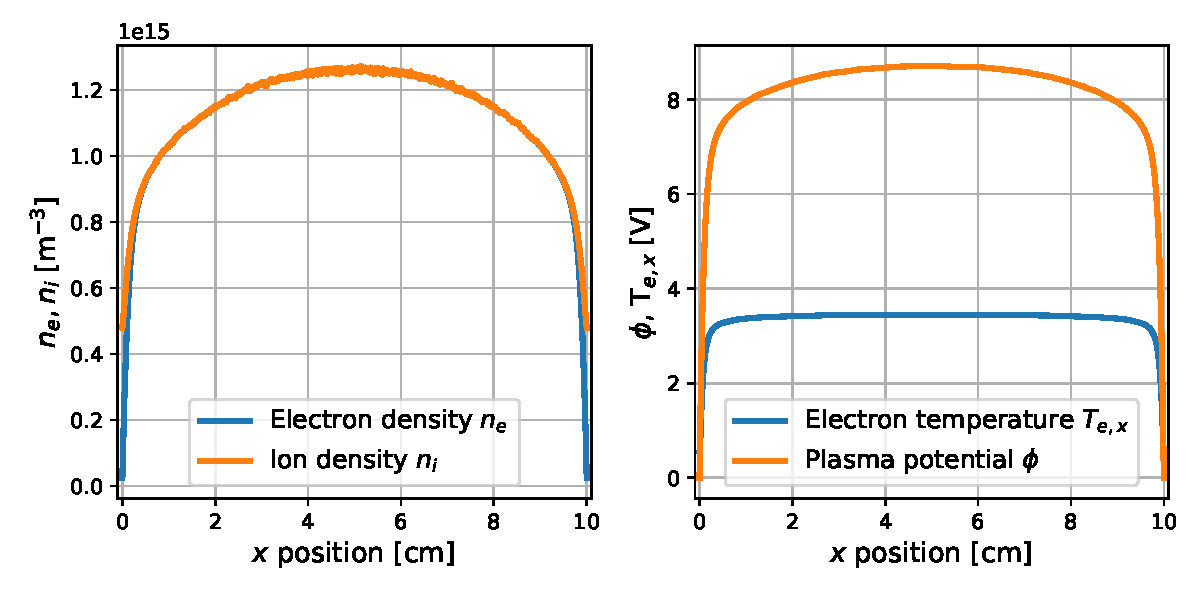
\includegraphics[width=0.9\textwidth]{ICP_results.pdf}
  \caption{Results of the PIC simulation for the model \M2, using RF inductive heating.}
  \label{fig-icpresults}
\end{figure}

\Cref{fig-icpresults} presents the simulation results for the electron density, plasma potential and electron temperature using the parameters of \Cref{tab-PIC2}.
We can see that the different variables (density, electron temperature and the plasma potential) are not much affected compared to \M1.

\begin{figure}[!htbp]
  \centering
  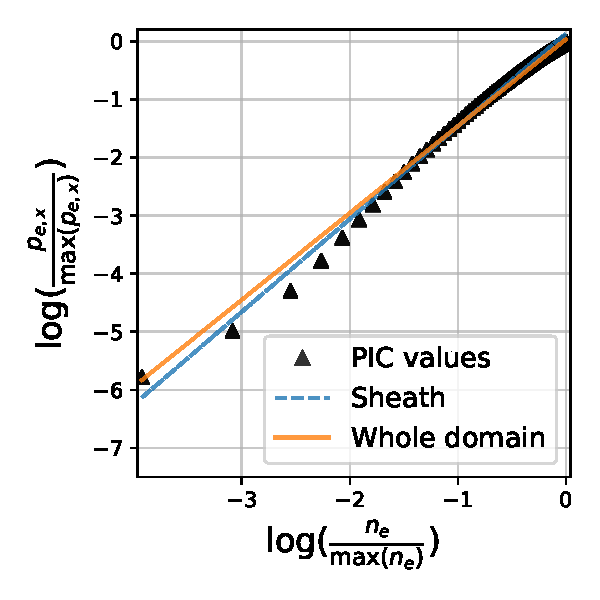
\includegraphics[width=\defaultwidth]{ICP_polyfit2.pdf}
  \caption{Estimation of the polytropic index in the sheath and in the whole domain in the PIC simulation using the model \M2.}
  \label{fig-icpfit}
\end{figure}

\Cref{fig-icpfit} presents the electron pressure as a function of the electron density measured in the simulation in log scale.
We see that the trend is not purely linear. Hence, the linear regression used in order to obtain the polytropic index is conducted twice\string:
\begin{itemize}
  \item In the whole domain\string: $\gamma=1.5$
  \item Only in the sheath\string: $\gamma=1.6$
\end{itemize}
The linear relation conducted of the whole domain is less precise than for the simulation result of \M1 ($R^2=0.992$).
However, we can see that the linear relation still describes quite well the electron evolution in the sheath.
The polytropic indexes obtained are close to the simulation using \M1 at the same pressure.

\begin{figure}[!htbp]
  \centering
  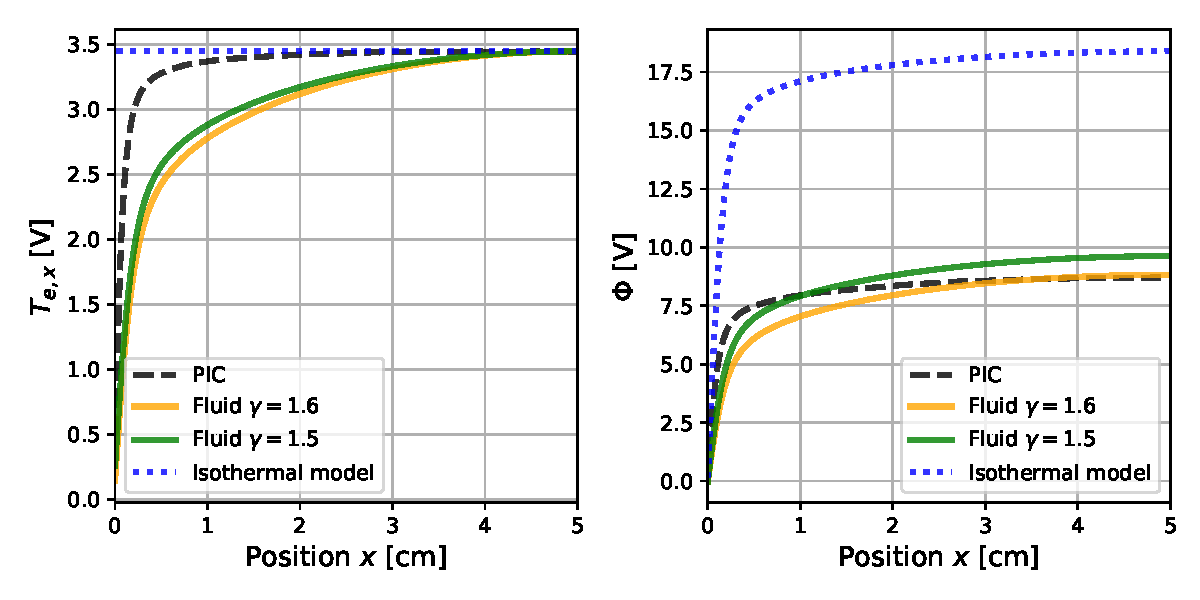
\includegraphics[width = 0.9\textwidth]{FluidComparisonICP.pdf}
  \caption{Comparison of the electron temperature and plasma potential measured in the PIC simulation with the prediction of the fluid model with $\gamma = 1.5$ (average index in the domain) and $\gamma=1.6$ (index in the sheath).}
  \label{fig-comp2}
\end{figure}

\Cref{fig-comp2} shows the comparison of the electron temperature and the plasma potential in the PIC simulation using the model  \M2 with the prediction of the fluid model of \cref{sec-fluid}.
We can see that the agreement between the PIC results and the fluid models is less satisfactory than in \cref{fig-comp} when using the model \M1, but it is still significantly better than the isothermal model.
Hence, even with a self-consistent heating and ionization in the plasma, the polytropic model stands as a better model for the sheath and the pre-sheaths.
